
This section deals two complementary scheduling strategies in detail with the performance plots to justify the claims. The first section discusses the capacity maximizing schemes discussed in section \ref{mtbus} with the assumption of zero pathloss between users and BS. The zero pathloss claim is assumed to bring out the scheduling schemes selection performance to maximize the sum capacity without which the all capacity seeking selection performs relatively closer with significant bias towards low pathloss users.
\begin{figure}
\centering
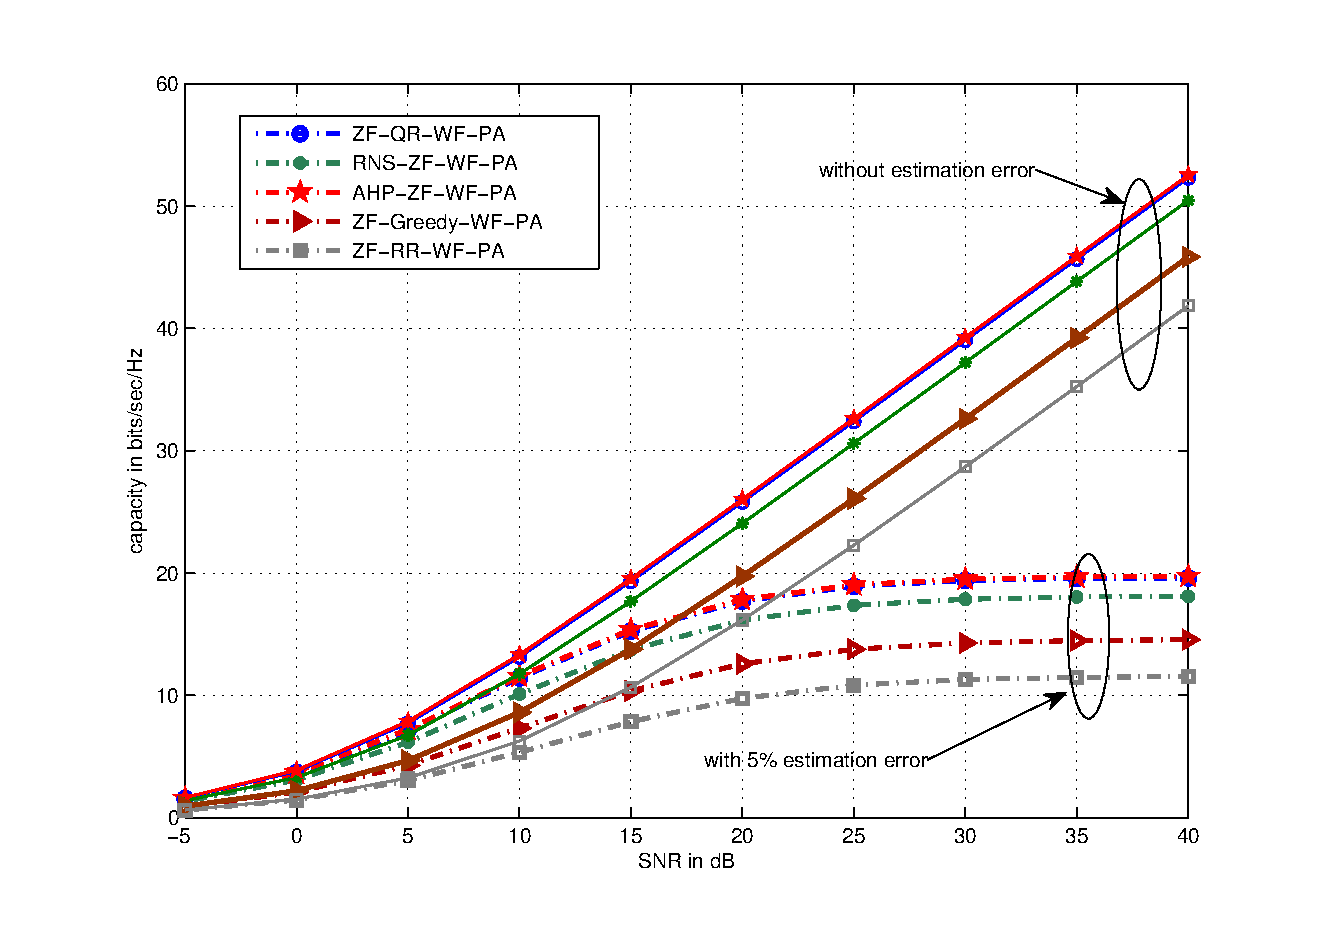
\includegraphics[width=0.8\textwidth]{single-bs-1}
\caption[short]{Sum capacity for \me{\card{\mc{U}} = 20, \, N_\mrm{T} = 4, \, N_\mrm{R} = 1}}
\label{single-bs-f1}
\end{figure}

Fig. \ref{single-bs-f1} compares the performance of capacity achieving user selection schemes discussed in section \ref{mtbus} to the QR based user selection scheme discussed in \cite{antti_user_selection,jin2010novel}. The AHP based user selection provides marginal but still noticeable performance improvement over the existing QR based algorithm. The gain is mainly attributed to the selection mechanism which takes pair-wise channel correlation metric in to account. This additional information is not of great value as it can be seen but the complexity involved in this is significantly large.
\begin{figure}
\centering
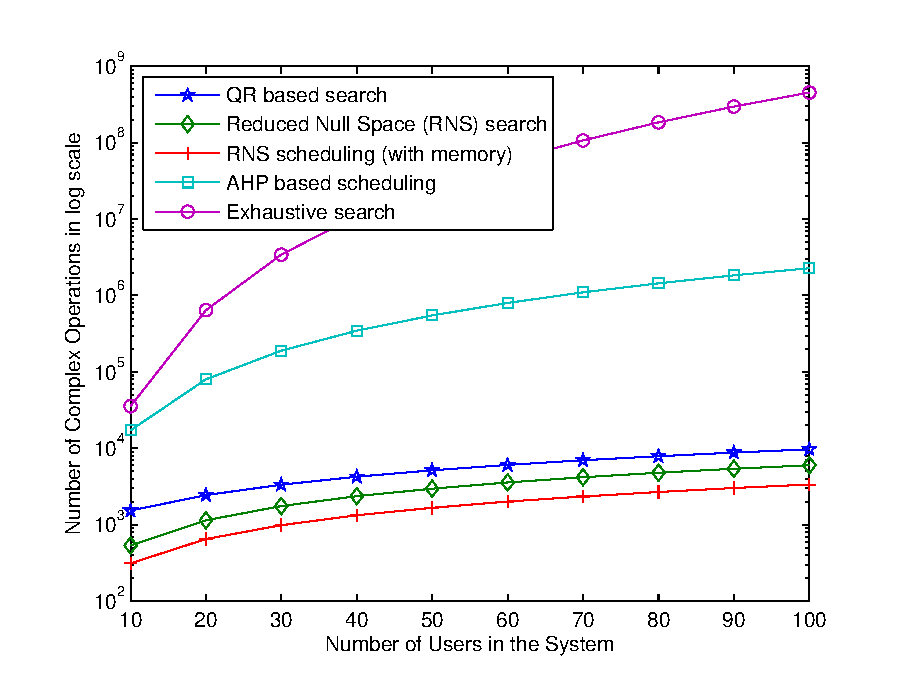
\includegraphics[width=0.8\textwidth]{single-bs-2}
\caption[short]{Scaling of complexity over users for \me{N_\mrm{T} = 4, \, N_\mrm{R} = 1} system}
\label{single-bs-f2}
\end{figure}

Fig. \ref{single-bs-f1} also shows the performance of reduced null space (RNS) scheme which performs closer to the existing QR algorithm but with huge reduction in the complexity involved in the metric calculation. Since QR based schemes requires matrix inverse computation for null space, RNS scheme provides a sub-optimal alternative to achieve the same. Fig. \ref{single-bs-f2} compares the complexity involved in performing various schemes discussed so far. The complexity involved in RNS user selection scheme is the least among the scheduling schemes based on channel correlation discussed here. The complexity can further be reduced by saving the earlier results in the memory (with some increase in the storage memory) to avoid redundant calculations over each iterations.
\begin{figure}
\centering
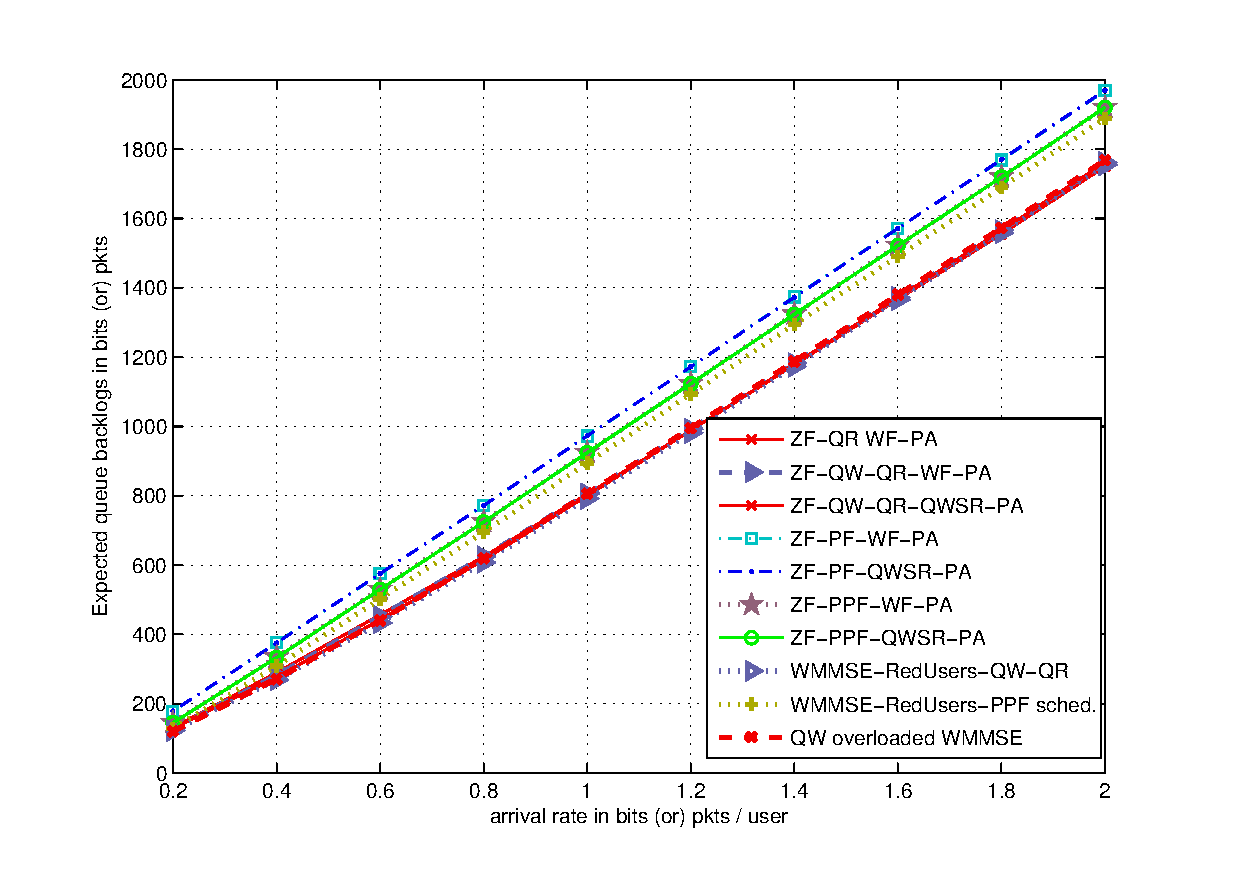
\includegraphics[width=0.8\textwidth]{single-bs-3}
\caption[short]{Expected queue size \me{\card{\mc{U}} = 50, \, N_\mrm{T} = 4, \, N_\mrm{R} = 1, \, \mc{U}(0,-30)} over \me{1000} slots at \me{15}dB SNR}
\label{single-bs-f3}
\end{figure}

Fig. \ref{single-bs-f1} depicts the performance degradation of above mentioned schemes with \me{5\%} estimation error modeled using Gaussian error. The estimation error degrades the performance by altering the precoders from being the perfect channel inverse there by creating interference among the transmitted streams. This effect is more pronounced at higher SNR as the capacity is starts saturating since the noise component is dominated by the interference in comparison with the AWGN.

The selection schemes discussed so far addresses the capacity achieving user selection schemes. Figs. \ref{single-bs-f3} and \ref{single-bs-f4} plots the performance of the selection schemes which minimizes the mean queue size and fairness among the users in the system. The users are associated with the uniform pathloss ranging in \me{\matscont{-30,0}} to analyze the fairness performance of user selection schemes. The power allocation scheme discussed earlier is used to achieve the objectives of fairness and queue backlogs reduction when the precoders are designed based on zero-forcing scheme. W-MMSE based scheme provides inherent power allocation for all the precoders based on the queue backlogs by maximizing the queue weighted sum rate objective. Fig. \ref{single-bs-f3} shows that the mean queue size is reduced by all schemes except few fairness based selection schemes like proportional fair (PF) and percentile PF (PPF) scheduling.
\begin{figure}
\centering
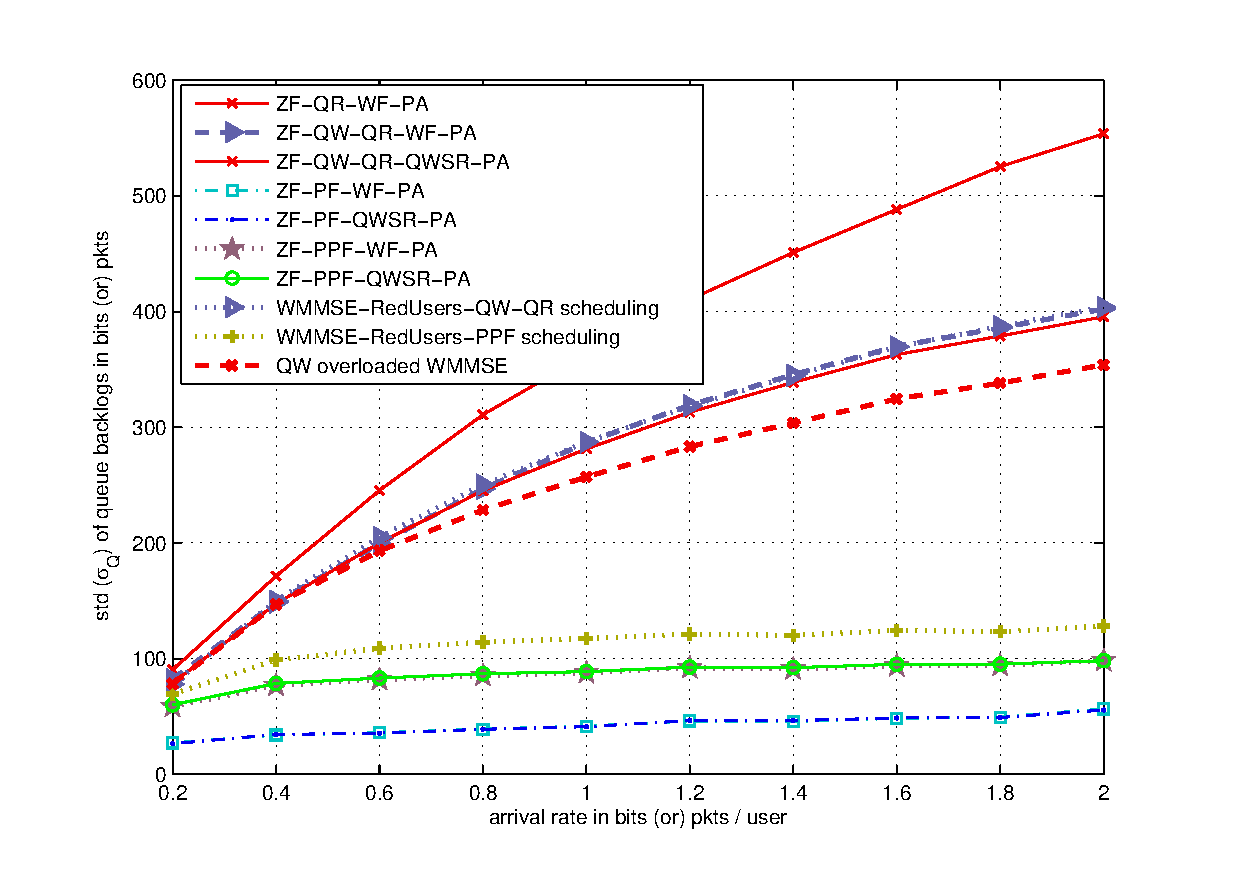
\includegraphics[width=0.8\textwidth]{single-bs-4}
\caption[short]{Standard deviation of backlogged packets \me{\card{\mc{U}} = 50, \, N_\mrm{T} = 4, \, N_\mrm{R} = 1, \, \mc{U}(0,-30)} over \me{1000} slots at \me{15}dB SNR}
\label{single-bs-f4}
\end{figure}

The PPF scheme provides significantly closer performance with the PF scheduling with better reduction in the average queue size. The computation of PPF scheduling is greatly reduced in comparison with other scheduling schemes since the QR based search is performed over \me{50 \%}ile users based on the PF metric as given by \eqref{qba2-e1}. The reduced user set allows users with PF metric significantly high to be searched for uncorrelated channels to form the set \me{\mc{S}} thereby achieving fairness among users.

The performance of queue weighted user selection with ZF precoding and queue weighted WF scheme \eqref{pa-e2} provides better fairness in comparison with the capacity achieving user selection and queue weighted selection with WF power allocation scheme \eqref{pa-e1} for the similar backlogged packet size. The fairness in the ZF scheme is achieved by the use of queue weighted power allocation strategy \eqref{pa-e2}. It is evident that the simple WF scheme \eqref{pa-e1} achieves fairness among user service in MU-MIMO with the queue weighted (QW) QR based scheme.

The overloaded W-MMSE case is plotted in Figs. \ref{single-bs-f3} and  \ref{single-bs-f4} along with other schemes for the comparison purpose. The plot shows that the performance of the overloaded W-MMSE scheme provides significantly fair selection in comparison with the ZF counterparts. The reduced W-MMSE scheme with the selection based on QW QR scheme provides fairness in comparison with the overloaded W-MMSE scheme by greatly reducing the computational complexity involved.
